\chapter{Pipeline Overview}\label{ch:pipeline-overview}
In this thesis, our goal is to build an End-to-End tool that takes in domain-expert knowledge from the ArduPilot community, extracts \ac{CEP}s, outputs a \ac{WDCG}, and evaluates the results.
We realize this by building a pipeline consisting of four modules depicted in \autoref{fig:pipeline-overview}.
This chapter will give a big picture of our complete architecture and show how the different modules are connected.

\begin{figure}
    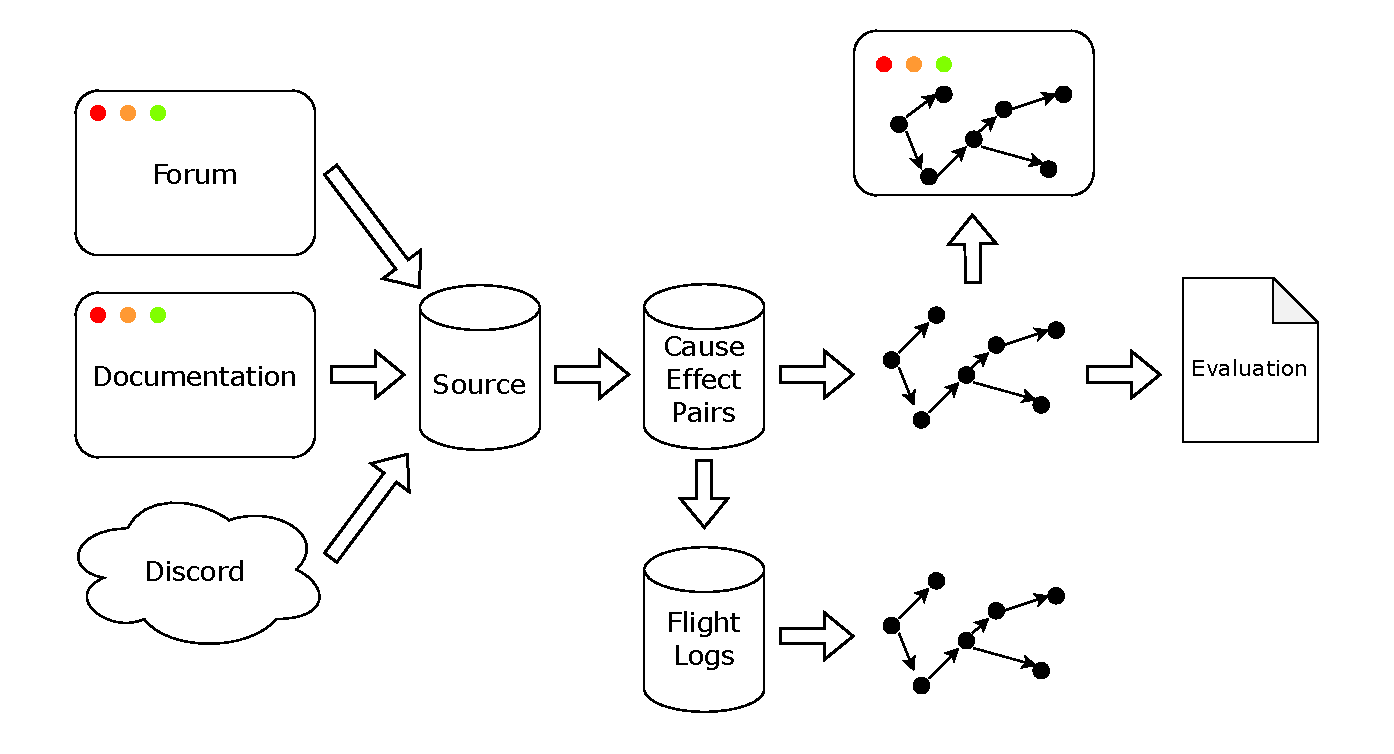
\includegraphics[width=\textwidth]{figures/pipeline_overview/pipeline_overview}
    \caption{End-to-End Pipeline Overview}\label{fig:pipeline-overview}
\end{figure}


\section{Data Collection}\label{sec:data-collection-pipeline}
The goal of this module is to provide a dataset which contains correct and cleaned sentences from domain-experts of the ArduPilot community.
We divided this module into four independent submodules to ensure an efficient and flexible scraping procedure.
The first three submodules gather raw text from the ArduPilot community channels: the discussion forum, the Discord chat, and the online documentation.
To gather the data from the different sources, we used the respective scraping techniques described in \autoref{subsec:evaluation-of-the-correct-technique}.
Next, we store the results from each module into an independent data storage, which can be filled either once when we run the pipeline from start to finish or by manually updating a specific data storage.
Finally, after we gathered the raw data from all sources, we extracted sentences from each source, gave each sentence a unique identifier, and combined the sentences into one dataset.


\section{Cause-Effect Pair Extraction}\label{sec:cause-effect-pair-extraction-pipeline}
This module takes the domain-expert sentences from the data collection module as input and outputs multiple \ac{CEP}s.
We first filter the sentences that contain explicitly mentioned causation and cache them in a dataset.
We then use this cached dataset to find \ac{CEP}s based on dependency patterns and phrase extraction techniques (see \autoref{subsec:scope-of-the-thesis}).
Finally, we store the extracted \ac{CEP}s for further processing.


\section{Causal Graph Generation}\label{sec:causal-graph-generation-pipeline}
This module consists of three submodules.
The first module takes the raw \ac{CEP}s from the previous module and transforms them into a \ac{WDCG} (see \autoref{sec:causal-graphs}).
The second module builds a \ac{WDCG} from the flight logs dataset.
We store the resulting nodes, edges, and weights for both \ac{WDCG} for further evaluation.
The last module provides an interactive tool for a \ac{WDCG} to explore the structure and trace events to root nodes back.


\section{Evaluation}\label{sec:evaluation-pipeline}
\begin{figure}
    \begin{center}
        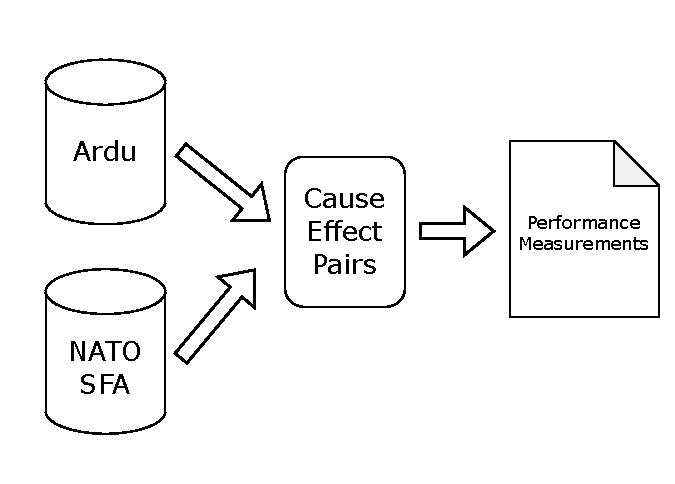
\includegraphics[scale=.7]{figures/pipeline_overview/evalutation_overview}
        \caption{Performance Measurement Overview}\label{fig:evaluation-overview}
    \end{center}
\end{figure}
The last module contains two submodules to evaluate the \ac{CEP} algorithm and the \ac{WDCG}.
The first submodule measures the performance of the \ac{CEP} extraction algorithm, which can be additionally seen in \autoref{fig:evaluation-overview}.
We use two labeled datasets to provide a domain-independent result, one from a foreign-domains and one was created from the domain-expert knowledge dataset from \autoref{sec:data-collection-pipeline}.
The second submodule analyses the \ac{WDCG} and infers the quality of the online resources.
Moreover, this submodule compares the causal graph with the flight logs graph generated in \autoref{sec:causal-graph-generation-pipeline}.
